%------------------------------------------------------------------------
%Editar Diplomado
\hypertarget{cv:eliminarAtributo}{\section{Eliminar Atributo}} \label{sec:eliminarAtributo}

	Esta funcionalidad le permitirá eliminar un atributo innecesaria o incorrecta. Para eliminar el atributo es necesario que no se encuentre asociado a casos de uso.
		\subsection{Procedimiento}

			%Pasos de procedimiento
			\begin{enumerate}
	
			\item Oprima el botón \IUBotonEliminar{} de un registro existente de la pantalla \ref{fig:GestionarAtributos} ''Gestionar Atributos''.
	
			\item Se mostrará el mensaje \ref{fig:confirmaEliminaAtributo} sobre la pantalla \ref{fig:GestionarAtributos} ''Gestionar Atributos''.
			
			%Pantalla
			\begin{figure}[htbp!]
				\begin{center}
					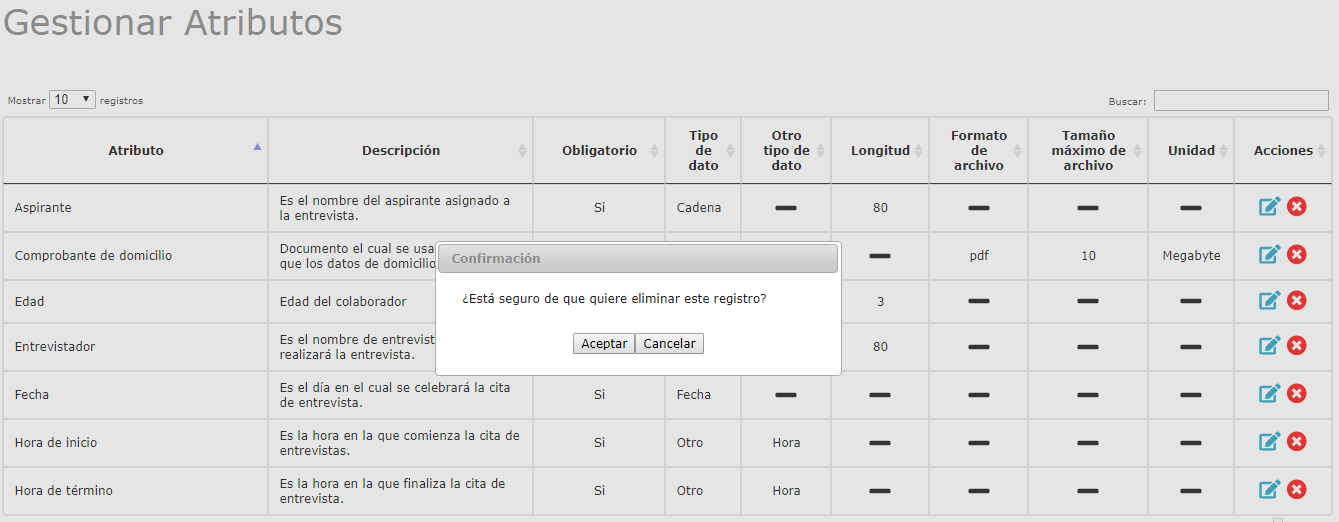
\includegraphics[scale=0.5]{roles/lider/entidades/atributos/pantallas/IU12-1-3MSG10}
					\caption{MSG de Confirmación}
					\label{fig:confirmaEliminaAtributo}
				\end{center}
			\end{figure}
						
			\item Oprima el botón \IUAceptar.
			
			\item Se mostrará el mensaje \ref{fig:atributoEliminado} en la pantalla \ref{fig:GestionarAtributos} ''Gestionar Atributos''.
			
			\begin{figure}[htbp!]
				\begin{center}
					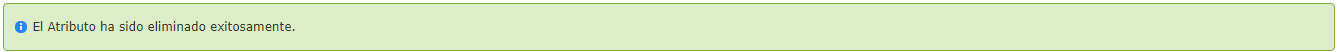
\includegraphics[scale=0.5]{roles/lider/entidades/atributos/pantallas/IU12-1-3MSG1}
					\caption{MSG: Atributo Eliminado}
					\label{fig:atributoEliminado}
				\end{center}
			\end{figure}
			\end{enumerate}